\begin{figure}[htbp]
    \centering
    \begin{subfigure}[t]{0.8\textwidth}
        \centering
        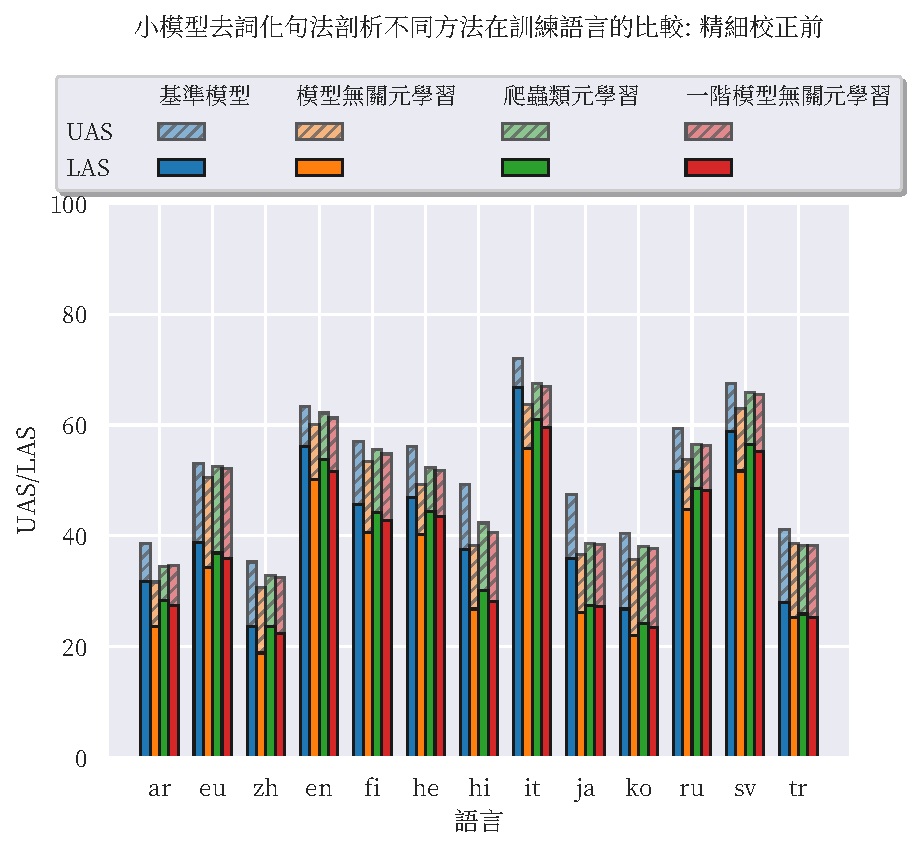
\includegraphics[width=\textwidth]{figs/delex_parsing/barplots/bar_small_zs_train_langs.pdf}
    \end{subfigure}
    \vspace{-12pt}
    \begin{subfigure}[t]{0.8\textwidth}
        \centering
        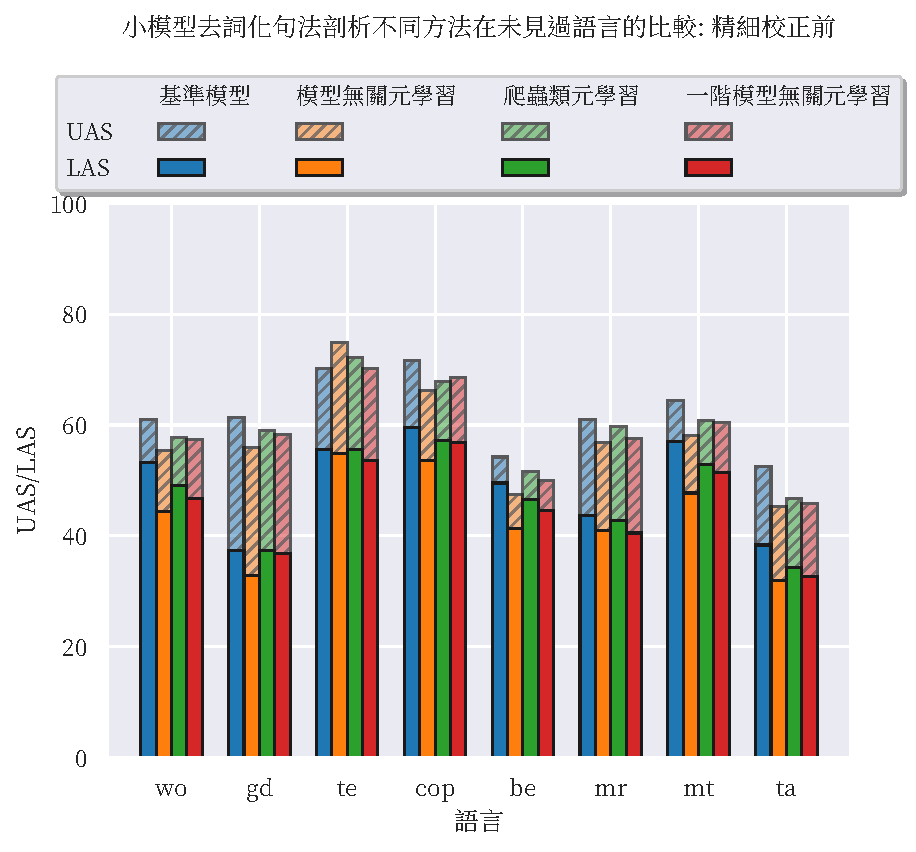
\includegraphics[width=\textwidth]{figs/delex_parsing/barplots/bar_small_zs_test_langs.pdf}
    \end{subfigure}
    \caption{小模型去詞化依存句法剖析不同方法在各語言精細校正前的UAS/LAS長條圖。}
    \label{fig:bar_small_zs}
\end{figure}
\begin{figure}[htbp]
    \centering
    \begin{subfigure}[t]{0.8\textwidth}
        \centering
        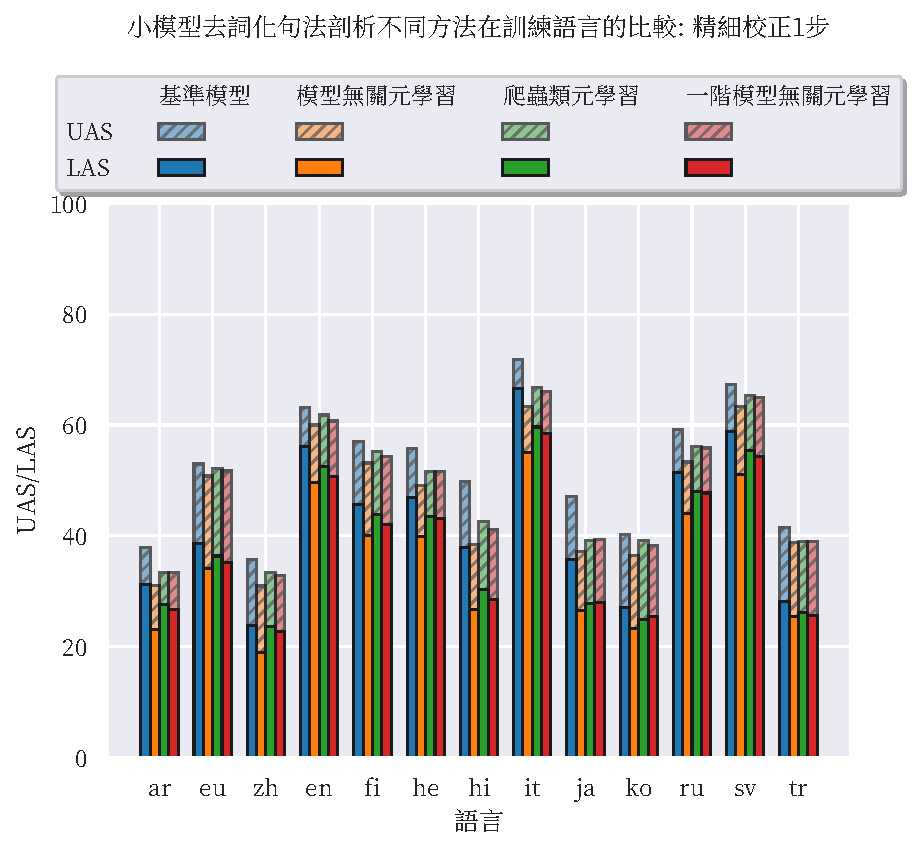
\includegraphics[width=\textwidth]{figs/delex_parsing/barplots/bar_small_one_step_train_langs.pdf}
    \end{subfigure}
    \vspace{-12pt}
    \begin{subfigure}[t]{0.8\textwidth}
        \centering
        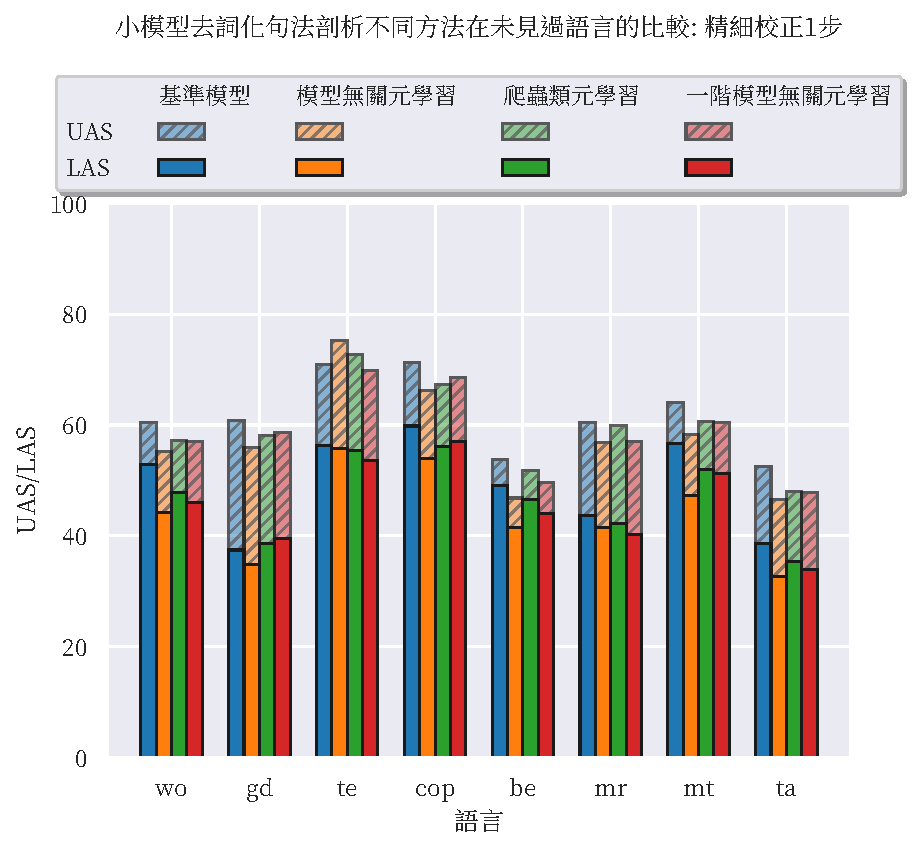
\includegraphics[width=\textwidth]{figs/delex_parsing/barplots/bar_small_one_step_test_langs.pdf}
    \end{subfigure}
    \caption{小模型去詞化依存句法剖析不同方法在各語言精細校正一步($\frac{1}{6}$回合)後的UAS/LAS長條圖。}
    \label{fig:bar_small_one_step}
\end{figure}
\begin{figure}[htbp]
    \centering
    \begin{subfigure}[t]{0.8\textwidth}
        \centering
        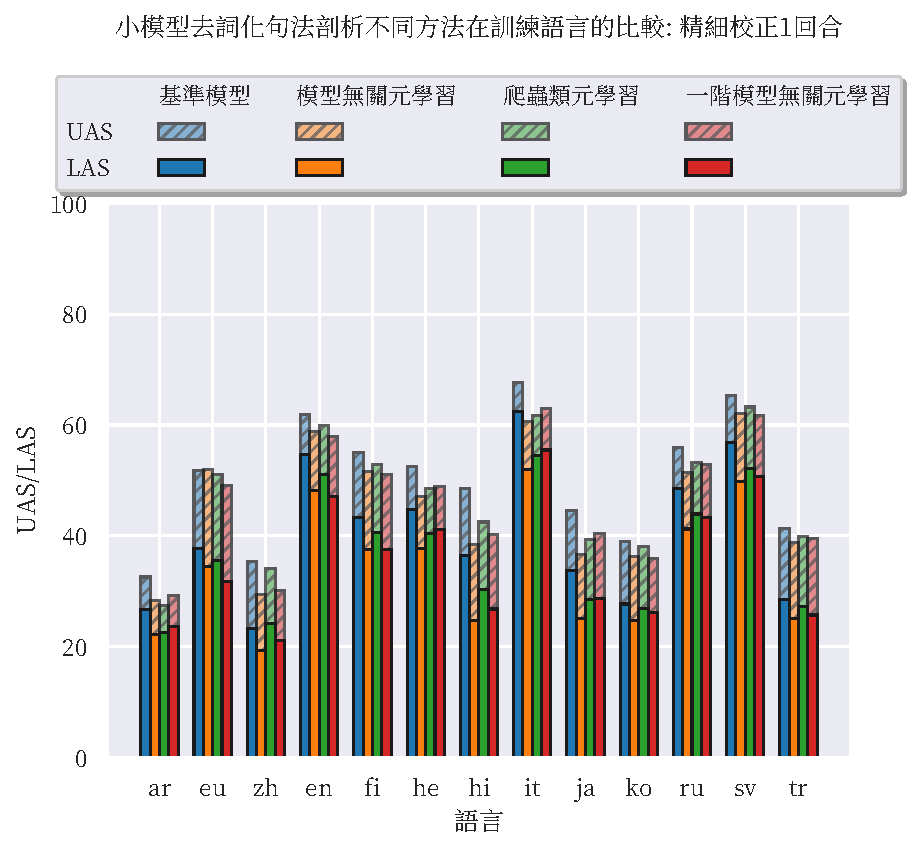
\includegraphics[width=\textwidth]{figs/delex_parsing/barplots/bar_small_full_epoch_1_train_langs.pdf}
    \end{subfigure}
    \vspace{-12pt}
    \begin{subfigure}[t]{0.8\textwidth}
        \centering
        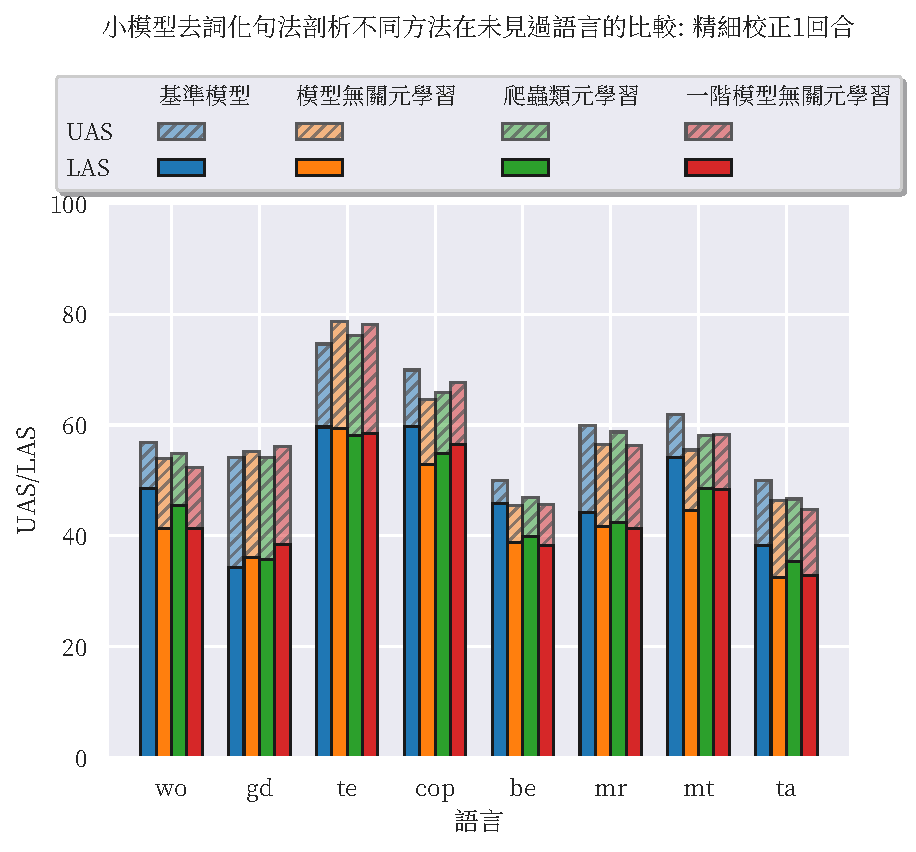
\includegraphics[width=\textwidth]{figs/delex_parsing/barplots/bar_small_full_epoch_1_test_langs.pdf}
    \end{subfigure}
    \caption{小模型去詞化依存句法剖析不同方法在各語言精細校正一回合後的UAS/LAS長條圖。}
    \label{fig:bar_small_full_epoch_1}
\end{figure}
\begin{figure}[htbp]
    \centering
    \begin{subfigure}[t]{0.8\textwidth}
        \centering
        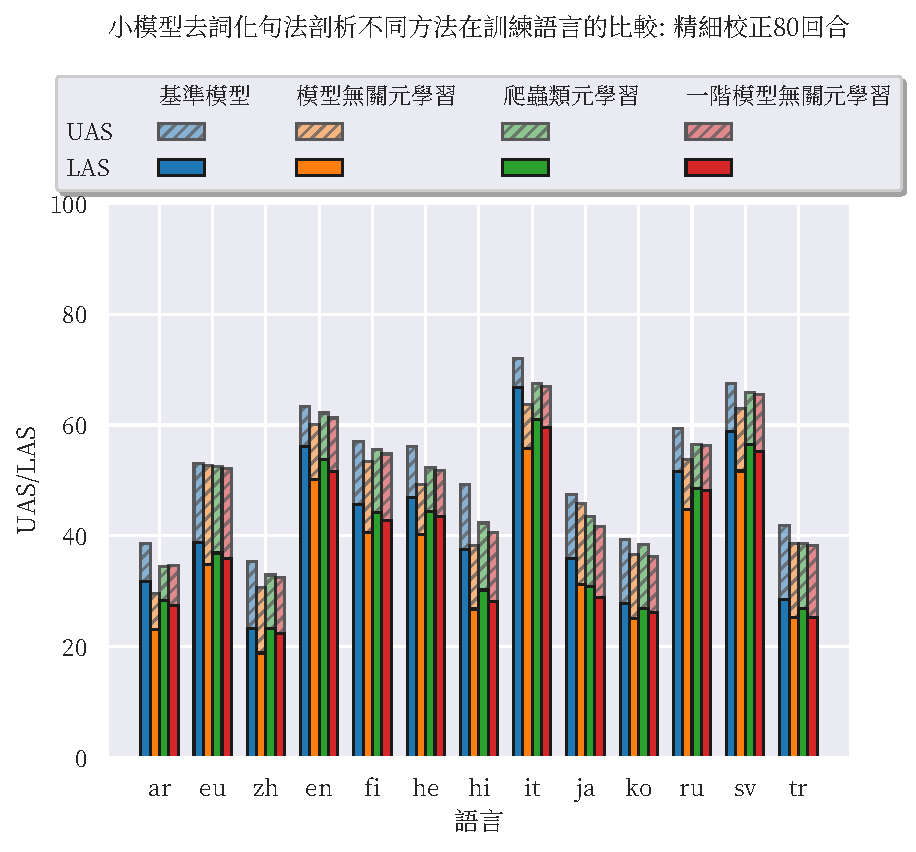
\includegraphics[width=\textwidth]{figs/delex_parsing/barplots/bar_small_full_epoch_80_train_langs.pdf}
    \end{subfigure}
    \vspace{-12pt}
    \begin{subfigure}[t]{0.8\textwidth}
        \centering
        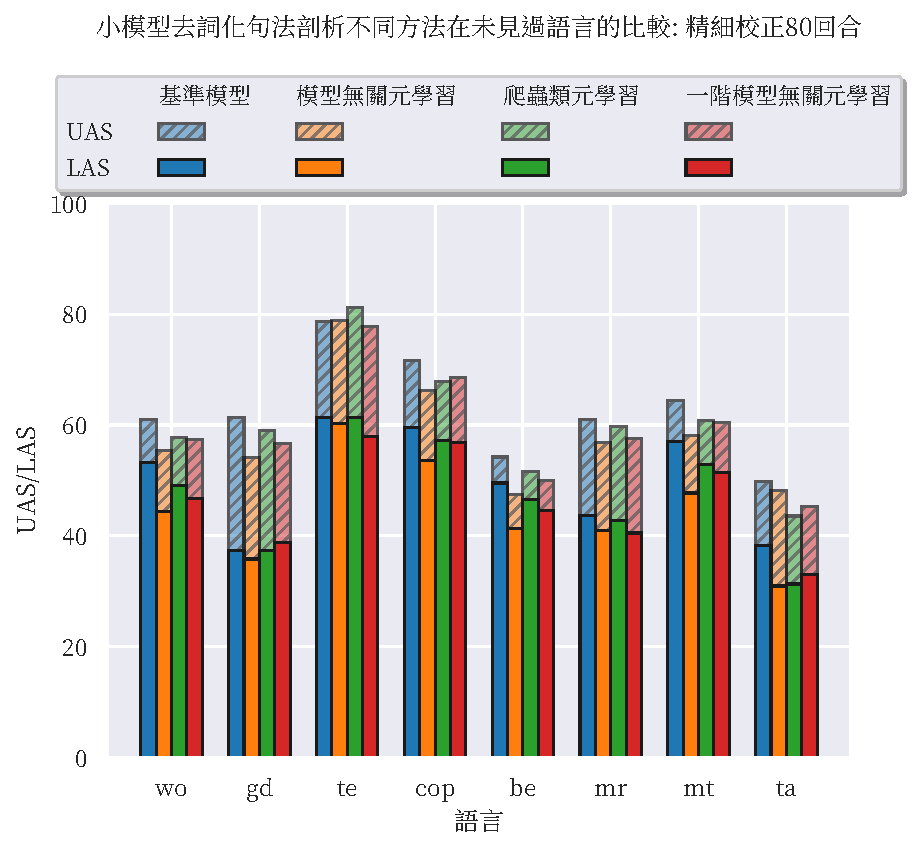
\includegraphics[width=\textwidth]{figs/delex_parsing/barplots/bar_small_full_epoch_80_test_langs.pdf}
    \end{subfigure}
    \caption{小模型去詞化依存句法剖析不同方法在各語言精細校正八十回合後的UAS/LAS長條圖。}
    \label{fig:bar_small_full_epoch_80}
\end{figure}
